\documentclass[dvipdfmx]{report} % 文章の形式を設定
\usepackage[margin=2.5cm]{geometry} % 書式の空白を設定
\usepackage[utf8]{inputenc} % 文字コードをUTF-8に設定
\usepackage{hyperref} % 目次にリンクを付けるため
\usepackage{lipsum} % ダミーテキスト用
\usepackage{tcolorbox} % 枠を利用するため
\usepackage{amsmath} % 数式の記述を行うため
\usepackage{bm} % ベクトルを太字で表示するため
\usepackage{graphicx} % 画像を表示するため
\usepackage{float} % 画像正しい位置で表示するため
\usepackage{tensor} % テンソルを記載するため
\usepackage{multicol} % 複数段落を作成するため
\usepackage{tikz} % 図を作成するため
\usepackage{amssymb} % 特殊文字を表示するため
\usepackage{enumerate} % リストを作成するため


\title{高密度コアを持つダークマター分布における近日点のシフト}
\author{Takahisa Igata, Yosuke Takamori}
\date{}

\begin{document}
\maketitle % タイトルの作成

\section*{概要}
本研究では、高密度コアを持つダークマター分布における近日点シフトを考察する。
ダークマターの分布を密度コアモデルで記述し、エネルギーパラメータがシステム全体で保存されることを仮定する。
このモデルでは、エネルギーパラメータの範囲に対して漸近的な解析を行い、周回運動の一般相対論的効果を示すほぼ円形の軌道を求めることができる。
これにより、近日点シフトにおいて、二つの競合する効果、すなわち曲率効果と局所的な密度効果が識別される。

さらに、漸近的な解析を用いることで、近日点シフトが局所的な密度効果を上回る領域が特定される。
この結果は、近日点シフトの存在が、一般相対論的効果を超えた物理的に合理的な物質の分布の存在を意味し、エキゾチックな天体(例えば、裸の特異点やワームホール)の存在を意味するのではないことを示唆する。
したがって、近日点シフトはブラックホールの代替モデル、例えばダークマターコアと純粋なブラックホールを区別する上で重要な役割を果たす。

DOI: 10.1103/PhysRevD.105.124029

\section*{II. Buchdahl時空}
Buchdahl時空を再検討する。本論では、計量は次式で与えられる。
\begin{equation}
    ds^2 = -\frac{(1-f)^2}{(1+f)^2} dt^2 + (1+f)^4 (dr^2 + r^2 d\theta^2 + r^2 \sin^2 \theta d\varphi^2)
\end{equation}
\begin{equation}
    f(r) = \frac{a}{2\sqrt{1 + kr^2}}
\end{equation}
ここで、$a$および$k$は定数である。
これらのパラメータの物理的解釈は、以下の式(12)および(14)で明確になる。
この空間的部分はユークリッド平坦計量に対して共形的に同型であり、標準的な球座標$(r, \theta, \varphi)$で表される。この計量は、静的かつ球対称性を認めるものである。
$a > 0$および$k > 0$と仮定する。
すると、関数$f$は中心$r = 0$で$f(0) = a/2 > 0$をとり、$r$が増加するにつれて単調に減少してゼロに近づく。ここで、$0 \leq r < \infty$である。

アインシュタイン方程式は、ストレス-エネルギーテンソルを持つ完全流体として物質分布を導く。ストレス-エネルギーテンソルは次のように与えられる。
\begin{equation}
    T_{ab} = \rho u_a u_b + p (g_{ab} + u_a u_b)
\end{equation}
ここで、$g_{ab}$は計量テンソルを表し、$u^a$は時空を満たす静的観測者の接ベクトル場を表す。また、
\begin{equation}
    \rho(r) = \frac{24k f^5}{\pi a^4 (1 + f)^5}
\end{equation}
\begin{equation}
    p(r) = \frac{8k f^6}{\pi a^4 (1 - f^2)(1 + f)^4}
\end{equation}
である。

エネルギー密度と圧力をそれぞれ$\rho$および$p$とし、$q$を次のように定義する。
\begin{equation}
    q = \frac{3p}{\rho} = \frac{f}{1 - f}
\end{equation}
式(4)および(5)から、流体の状態方程式を得ることができる。
\begin{equation}
    \frac{p}{p_c} = \frac{(\rho/\rho_c)^{6/5}}{1 + 2q_c[1 - (\rho/\rho_c)^{1/5}]},
\end{equation}
ここで、$\rho_c$、$p_c$、$q_c$はそれぞれ、中心$r = 0$における$\rho$、$p$、および$q$の値である。それらは次のように与えられる。
\begin{equation}
    \rho_c = \frac{24ak}{\pi (2 + a)^5}
\end{equation}
\begin{equation}
    p_c = \frac{8a^2k}{\pi (2 - a)(2 + a)^5}
\end{equation}
\begin{equation}
    q_c = \frac{a}{2 - a}
\end{equation}

$q_c \ll 1$(すなわち、$a \ll 1$)の場合、状態方程式(7)は多項式指数5の多項式方程式に簡約され、重力ポテンシャル、エネルギー密度、および圧力はニュートン的Plummerモデルのものと一致する。したがって、このモデルは一般相対論的Plummerモデルとして知られている。

物質場にエネルギー条件を課すことで、解のパラメータ領域がさらに制限される。いくつかのエネルギー条件は以下のように記述される:
\begin{enumerate}[(i)\,]
    \item 弱エネルギー条件: $\rho \geq 0$ および $\rho + p \geq 0$。
    \item 強エネルギー条件: $\rho + 3p \geq 0$ および $\rho + p \geq 0$。
    \item 無エネルギー条件: $\rho + p \geq 0$。
    \item 優勢エネルギー条件: $\rho \geq |p|$。
\end{enumerate}

$a \leq 2$ の場合、$\rho$ と $p$ は全領域で非負であり、弱エネルギー、強エネルギー、無エネルギー条件を満たす。一方、$3/2 < a \leq 2$ では少なくとも中心付近では優勢エネルギー条件が成立しないが、$a \leq 3/2$ の場合、全領域で優勢エネルギー条件を満たす。そのため、$a \leq 3/2$ と仮定し、全領域でのすべてのエネルギー条件を満たす。

半径$r$以内の適切質量を次のように定義する。
\begin{equation}
    m(r) = \int_0^r \rho(\xi) \sqrt{h} d^3x = \frac{akr^3}{(1 + kr^2)^{3/2}}
    + \frac{3a^2}{16\sqrt{k}} \left[ \arctan(\sqrt{kr}) - \frac{\sqrt{kr}(1 - kr^2)}{(1 + kr^2)^2} \right]
\end{equation}
ここで、$\Phi = -2f = -\frac{a}{\sqrt{1 + kr^2}}$、$\rho = \frac{3ka}{4\pi(1 + kr^2)^{5/2}}$、$p = \frac{a^2k}{8\pi(1 + kr^2)^3}$である。$\Phi$はニュートン的重力ポテンシャルに対応する。

$\sqrt{h} d^3x = \xi^2 [1 + f(\xi)]^6 \sin \theta d\xi d\theta d\varphi$は静的超曲面上の3次元体積要素である。したがって、全適切質量は次のように与えられる。
\begin{equation}
    M = \lim_{r \to \infty} m(r) = \frac{a}{\sqrt{k}} \left( 1 + \frac{3\pi a}{32} \right).
\end{equation}

面積半径$\tilde{r}$を導入する。この半径は$r$よりも物理的な解釈が明確であり、次のように定義される。
\begin{equation}
    \tilde{r} = r (1 + f)^2.
\end{equation}

コアスケール$r = 1/\sqrt{k}$における$\tilde{r}$を評価して、コア半径$R$を次のように定義する。
\begin{equation}
    R = \tilde{r} \bigg|_{r = 1/\sqrt{k}} = \frac{1}{\sqrt{k}} \left( 1 + \frac{a}{2\sqrt{2}} \right)^2.
\end{equation}

$\tilde{r} \leq R$の領域をコアと呼び、比$M/R$をコアのコンパクトさとする。この比は$a$に単調に依存し、$a \ll 1$の場合には$a$に減少するため、$a$自体をコンパクトさと緩やかに参照する。図1は、正規化された面積半径$\tilde{r}/R$に対する$\rho/\rho_c$および$m/M$の関数としてそれぞれ示している。これらの図は、このモデルの質量分布がコア半径$R$の内部、特に中心付近に局在していることを示唆している。コンパクトさが小さい場合(すなわち、$a \ll 1$)、$\rho$および$m$の値は依然として以下の値をとる。

次の関係式が成り立つ。
\begin{equation}
    \left. \frac{\rho}{\rho_c} \right|_{r = 1/\sqrt{k}} = \left( \frac{2 + a}{2\sqrt{2} + a} \right)^5 \simeq \frac{1}{4\sqrt{2}} = 0.1767\ldots,
\end{equation}
\begin{equation}
    \left. \frac{m}{M} \right|_{r = 1/\sqrt{k}} \simeq \frac{1}{2\sqrt{2}} = 0.3535\ldots.
\end{equation}

システムがよりコンパクトになる、すなわちコンパクトさが増加するにつれて、これらの値もそれに応じて増加する。


\newpage
\section{メモ用}
/////////////////////////////////////////////////////////////////////////\\
/////////////////////////////////////////////////////////////////////////

% 方程式
\begin{equation*}
\begin{split}
	\bar{w}_j = \left( \right) \int^{}_{}
\end{split}
\end{equation*}

% ボックス
\begin{tcolorbox}[title=メモ用]
\[ 1 = 1 \]
\end{tcolorbox}

% { 付き方程式
\begin{equation}
\left\{ \,
\begin{aligned}
	1 &= 0\\
	1 &= 0\\
\end{aligned}
\right.
\end{equation}

% 画像
% \begin{figure}[H]
%    \centering
%     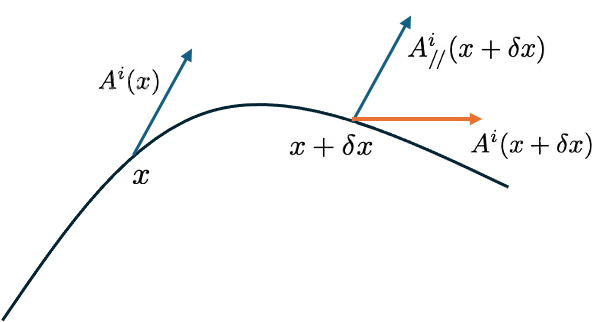
\includegraphics[width=0.5\columnwidth]{./images/0106/01.png}
%     \caption{並行移動}
%     \label{}
% \end{figure}

% リスト
\begin{enumerate}[(1)\,]
\item{}
\end{enumerate}

\end{document}